\begin{frame}
  \frametitle{\problemtitle}
  \begin{block}{Problem}
    Find and interactively execute a winning strategy in the following game:
    \begin{itemize}
      \item There are some cards containing math operations $+ n$ and $\times n$.
      \item Two players alternate picking cards until no cards are left.
      \item These operations are applied to a given number in the order they are picked.
      \item One player wins if the final result is even, the other wins if it is odd.
    \end{itemize}
  \end{block}
  \centering
  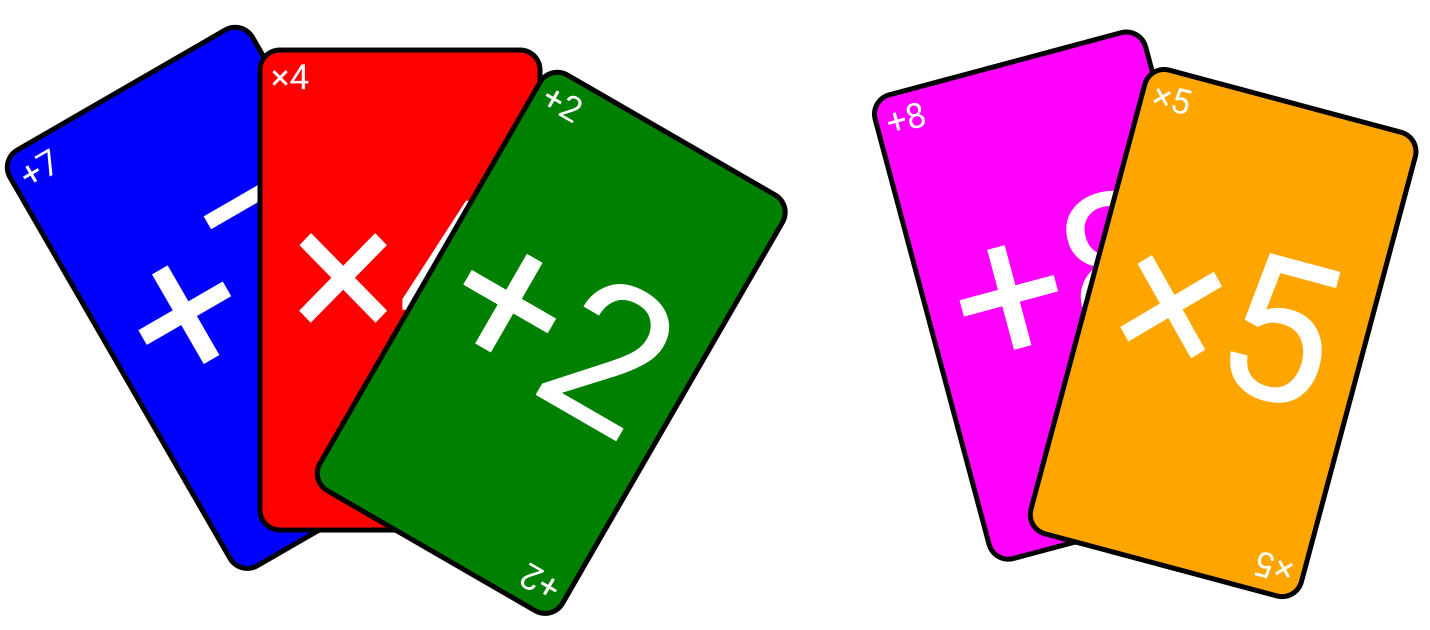
\includegraphics[width=0.6\textwidth]{cards.png}
\end{frame}
\begin{frame}
  \frametitle{\problemtitle}
  \begin{block}{Solution}
    \begin{itemize}
      \item<+-> As we only care about parity, reduce all numbers $\mathsf{mod}\;2$.
      \item<+-> So there are only three types of cards: $+0$, $+1$, $\times 0$
        \begin{itemize}
          \item Note that $+0$ is the same as $\times 1$.
        \end{itemize}
      \item<+-> There are at most $n \le 300$ cards, so we can use $\Theta(n^3)$ dynamic programming:
        \begin{equation*}
          \texttt{dp[who][cur][a][b][c]} =
            \begin{array}{l}
              \text{Does player \texttt{who} win when the current value is \texttt{cur} and there} \\
              \text{are \texttt{a}, \texttt{b} and \texttt{c} operations of the respective types remaining?}
            \end{array}
        \end{equation*}
      \item<+-> The game can be played by following along the values in the DP table.
    \end{itemize}
  \end{block}
  \pause
  \begin{block}{Challenge}
    Can you also solve the problem for $n \le 10^5$?
  \end{block}
\end{frame}
